\documentclass[a4paper,11pt]{article}
\usepackage[utf8]{inputenc}
\usepackage[T1]{fontenc}
\usepackage{graphicx}
\usepackage{geometry}
\usepackage[colorlinks,linkcolor=black,urlcolor=cyan,citecolor=cyan]{hyperref}
\usepackage{amsmath}
\usepackage{fancyhdr}
\usepackage{float}
\usepackage{listings}
\usepackage{tikz}
\usepackage{animate}
\usepackage{tcolorbox}
\usepackage{xcolor}
\usepackage[french]{babel}

\geometry{left=3cm,right=3cm,top=2.5cm,bottom=2.5cm}

\hypersetup{
    colorlinks=true,
    linkcolor=black,
    urlcolor=cyan,
    citecolor=cyan
}

\lstset{
    language=Fortran,
    basicstyle=\tiny,
    keywordstyle=\color{blue}\bfseries,
    commentstyle=\color{gray},
    stringstyle=\color{red},
    numbers=left,
    numberstyle=\tiny\color{gray},
    stepnumber=1,
    breaklines=true,
    frame=single,
    captionpos=b,
    tabsize=4,
    showstringspaces=false,
}

\begin{document}



\begin{titlepage}
    \begin{figure}
        
\includegraphics[width=0.4\linewidth]{images/logo_em.jpg}
    \end{figure}
    \begin{center}
        \vspace*{3.5cm}


        \huge \textbf{Travail d'étude et de Recherche} \\
        Compte rendu du semestre 6
        \vspace{1cm}

        \hrulefill
        
        \vspace{0.4cm}
        {\Huge \textbf{Modélisation du transfert thermique et de masse dans la pyrolyse du bois}} \\
        \vspace{0.25cm}
        \hrulefill

        \vspace{1cm}
        \normalsize
        
        \textbf{Participants :}
        Simon Francheo, Julien Léger, Gurwan Le Hebel, Pierre Mériaux
        \vspace{6cm}

        \Large Année Universitaire 2024 - 2025
        
        \vspace{2cm}
        
        
        \normalsize
        \textbf{Encadrants :}
        Ludovic Godard-Cadillac, Thanh-Ha Nguyen-Bui 

        \vfill
        
    \end{center}
\end{titlepage}

\newpage
\tableofcontents
\newpage

\pagestyle{fancy}
\fancyhead{}
\fancyhead[L]{TER - Pyrolyse du bois}
\fancyhead[R]{23 Janvier 2025}


\section{Introduction}
La construction d'un modèle de comportement de la pyrolyse du bois est un enjeu pour la sécurité incendie en forêt et pour les constructions. Ce modèle doit permettre le bon dimensionnement des structures en anticipant la formation d'une couche de charbon isolante autour du bois sain. 
\\

Le modèle que nous étudions utilise le couplage d'une modélisation des réactions chimiques de pyrolyse et d'une modélisation de la diffusion de la chaleur. La \nameref{sec:theo} présente les hypothèses et les équations utilisées. La résolution des équations sur les masses volumiques est ensuite effectuée en comparant les schémas Euler implicite et Crank-Nicolson. Le choix de schémas implicites est dû à des raisons de stabilité, d'absence de condition CFL contraignante sur le pas de temps et est facilité par la possibilité d'inverser analytiquement le schéma. Concernant la résolution de l'équation de la chaleur, un schéma numérique implicite est choisi, résultant d'un compromis entre temps de calcul et stabilité du schéma. Enfin, le couplage est effectué avec Euler implicite et Crank-Nicolson à 3 points, en 1D et en 2D.


\section{Partie théorique}\label{sec:theo}
\subsection{Équations de conservation de la masse}
La réaction de pyrolyse est modélisée par un système d'équations différentielles qui repose sur la conservation de masse du bois \cite{1}, du charbon, du gaz, du liquide et de la vapeur au cours du processus. Il s'écrit comme suit :
\begin{equation}\label{eq:1}
	\left\lbrace
		\begin{aligned}
			\frac{\partial \rho_b}{\partial t} &= -(k_1 + k_2)\rho_b \\
                \frac{\partial \rho_c}{\partial t} &= k_1\rho_b\\
                \frac{\partial \rho_g}{\partial t} &= k_2\rho_b\\
                \frac{\partial \rho_l}{\partial t} &= -k_3\rho_l\\
                \frac{\partial \rho_v}{\partial t} &= k_3\rho_l\\
		\end{aligned}
	\right.
\end{equation}

où $\rho_b, \rho_c, \rho_g, \rho_l, \rho_v$ sont respectivement les masses volumiques du bois, du charbon, du gaz, du liquide et de la vapeur.

$k_1, k_2, k_3$ sont les taux de réactions chimiques de la pyrolyse du bois humide. Ceux-ci sont décrits par la loi d'Arrhenius \cite{1}: 
\begin{equation}\label{eq:2}
    k_i = A_i\exp{\left(\frac{-E_i}{RT}\right)}, i = 1,2,3
\end{equation}

où $A_i$ sont des constantes de réactions, $E_i$ les énergies d'activation, R la constante des gaz parfaits et enfin T la température.

L'objectif est de résoudre ce système d'équations numériquement grâce à différents schémas implicites. Les applications numériques seront réalisées à partir de différentes essences de bois mouillés (cf \cite{1}). La relation suivante permet à partir des données brutes sur l'essence de bois étudiée d'extraite les masses volumiques $\rho_{b_0}$ et $\rho_{l_0}$ initiale \cite{1}.

\begin{equation}\label{eq:3}
    \rho_0 = (1 - \chi)\rho_{b_0} + \chi\rho_{l_0}
\end{equation}

où $\rho_0$ est la masse volumique du bois sec, et $\chi$ le taux d'humidité du bois. \\


Pour impliciter nos schémas numériques, il faut remarquer que les variations de $\rho_c, \rho_g$ sont dépendants uniquement de $\rho_b$, même chose pour $\rho_v$ qui dépend de $\rho_l$. Il faut inverser les équations pour $\rho_b$ et $\rho_l$ afin d'en déduire les autres avec les formules usuelles du schéma choisi. Les schémas sont alors partiellement implicites. Cette technique permet par exemple d'éviter l'utilisation de la méthode de Newton qui est très exigeante en temps de calcul. Le schéma numérique de Euler implicite s'écrit alors comme suit pour résoudre le système \eqref{eq:1}:

\begin{equation}\label{eq:EI}
	\left\lbrace
		\begin{aligned}
			\rho_b^{n+1} &=  \frac{\rho_b^n}{1 + \Delta t(k_1^{n+1}+k_2^{n+1})} \\
                \rho_c^{n+1} &= \rho_c^n + \Delta t \cdot k_1^{n+1} \rho_b^{n+1}\\
                \rho_g^{n+1} &= \rho_g^n + \Delta t \cdot k_2^{n+1}\rho_b^{n+1}\\
                \rho_l^{n+1} &= \frac{\rho_l^n}{1 + \Delta t \cdot k_3^{n+1}} \\
                \rho_v^{n+1} &= \rho_v^n + \Delta t \cdot k_3^{n+1} \rho_l^{n+1} \\
		\end{aligned}
	\right.
\end{equation}


Inversé analytiquement, le schéma de Crank-Nicolson implicite pour notre système s'écrit :

\begin{equation}\label{eq:CK}
	\left\lbrace
		\begin{aligned}
			\rho_b^{n+1} &= \rho_b^n \left( \frac{1 - \frac{\Delta t}{2}(k_1^n + k_2^n) }{1 +\frac{\Delta t}{2}(k_1^{n+1} + k_2^{n+1}) }\right)  \\
                \rho_c^{n+1} &= \rho_c^n + \frac{\Delta t}{2} \left( k_1^{n+1} \rho_b^{n+1} + k_1^n \rho_b^n \right) \\
                \rho_g^{n+1} &= \rho_g^n + \frac{\Delta t}{2} \left( k_2^{n+1} \rho_b^{n+1} + k_2^n \rho_b^n \right) \\
                \rho_l^{n+1} &= \rho_l^n \left(\frac{ 1 - \frac{\Delta t}{2} \cdot k_3^n }{ 1 + \frac{\Delta t}{2} \cdot k_3^{n+1} }\right)  \\
                \rho_v^{n+1} &= \rho_v^n + \frac{\Delta t}{2} \left( k_3^{n+1} \rho_l^{n+1} + k_3^n \rho_l^n \right) \\
		\end{aligned}
	\right.
\end{equation}
\subsection{Équation de la chaleur}
L'équation de la chaleur s'écrit :
\begin{equation}
    \rho C_{p} \frac{\partial T}{\partial t}=\frac{\partial}{\partial x}\left(\lambda \frac{\partial T}{\partial x}\right)+Q_{r}
\end{equation}
où $\lambda$, $\rho$ et $C_p$ sont respectivement le coefficient de conductivité thermique, la densité, la chaleur spécifique .

$Q_r$ est défini comme suit ($\Delta h_k^0$ la k-ième enthalpie de réaction) :
\begin{equation}
    \begin{aligned}
Q_{r} & =k_{1} \rho_{b}\left[\Delta h_{1}^{0}+\left(C_{c}-C_{b}\right)\left(T-T_{0}\right)\right] \\
& +k_{2} \rho_{b}\left[\Delta h_{2}^{0}+\left(C_{g}-C_{b}\right)\left(T-T_{0}\right)\right] \\
& +k_{3} \rho_{l}\left[\Delta h_{3}^{0}+\left(C_{v}-C_{l}\right)\left(T-T_{0}\right)\right] .
\end{aligned}
\end{equation}
La conductivité thermique équivalente du solide $\lambda_s$ s'écrit
\begin{equation}
    \lambda_s = \eta \lambda_c + (1-\eta)\lambda_b
\end{equation}
avec $\lambda_c$ conductivité du bois et $\lambda_b$ celle du charbon, estimée en tenant compte de l'effet de l'humidité $X$ :

\begin{equation}
    \begin{array}{l}
\lambda_{b}=0.166+0.369 X, \\
\lambda_{c}=0.105, \\
\eta = \frac{\rho_c}{\rho_s} = \frac{\rho_c}{\rho_c + \rho_b}
\end{array}
\end{equation}
\section*{Résultats et interprétations}\label{sec:ri}


\section{Partie chimie}
 
\subsection{Résolution numérique}

Pour obtenir les résultats, le temps maximal d'étude a été fixé à 300s (5 minutes), temps suffisant pour que toutes les transformations chimiques se produisent. Une température variant linéairement au cours du temps est choisie afin de ne pas compliquer le système. Cette température varie de 300K (température ambiante) à 1000K (727 °C) au cours de la réaction, permettant la visualisation de chaque transformation chimique en fonction de la température. Les taux de réactions chimiques k varient en même temps que la température, ce qui est décrit par la loi d'Arrhenius \eqref{eq:2}. En ce qui concerne la discrétisation du temps pour notre schéma numérique, le pas de temps est fixé à 0.1 s. Celui-ci est suffisamment petit pour avoir des résultats fiables (surtout avec Crank Nicolson), tout en garantissant un temps de calcul presque instantané. Le nombre d'itérations nécessaires pour le schéma N est donc de 3000. 
\\

L'essence de bois étudiée pour la résolution est principalement le Chêne de Mongolie (cf \cite{1}), celui-ci étant représentatif des charpentes utilisées dans les habitations, il est donc intéressant de le modéliser pour la prévention des incendies. \\

Pour un schéma donné, le programme principal stocke les données du problème et écrit les masses volumiques à chaque instant de notre subdivision. Cela est possible grâce à une boucle qui actualise successivement la température - donc les taux de réactions \eqref{eq:2} - et calcule les masses volumiques au temps n+1. Enfin, un script Gnuplot est utilisé pour tracer ces données :

\begin{figure}[H]
    \centering
    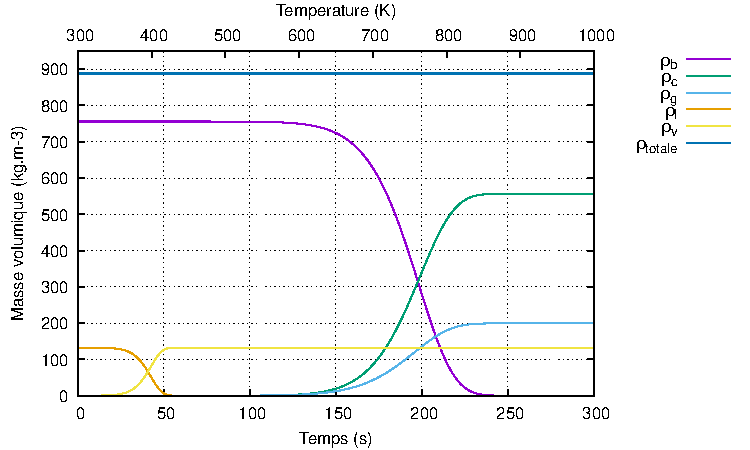
\includegraphics[width=0.8\linewidth]{images/densite_CK2.pdf}
    \caption{Évolution des masses volumiques en fonction du temps (et de la température) avec le schéma numérique de Crank Nicolson implicite }
    \label{fig:densiteCK2}
\end{figure}

L'évolution des masses volumiques correspond aux attentes suggérées par l'intuition physique. En effet, se produit dans un premier temps la vaporisation de l'eau (croisement des courbes de $\rho_l$ et $\rho_v$) autour de 100 °C. Celle-ci est suivie par la combustion, qui débute aux alentours de 600K, et qui est caractérisée par la transformation du bois en charbon et en gaz. De plus, la masse volumique totale reste stable tout au long de l'expérience. Ces observations confirment le bon comportement qualitatif du modèle.

\subsection{Étude de l'erreur}

Pour évaluer l'évolution de l'erreur locale d'un schéma en fonction du temps, on peut comparer deux solutions : l'une obtenue avec le schéma classique et l'autre avec le même schéma, mais en utilisant un pas de temps réduit, par exemple divisé par 10 (donc plus précis). L'écart absolu entre ces deux solutions à un instant donné t fournit une estimation de l'erreur locale du schéma.

\begin{figure}[H]
    \centering
    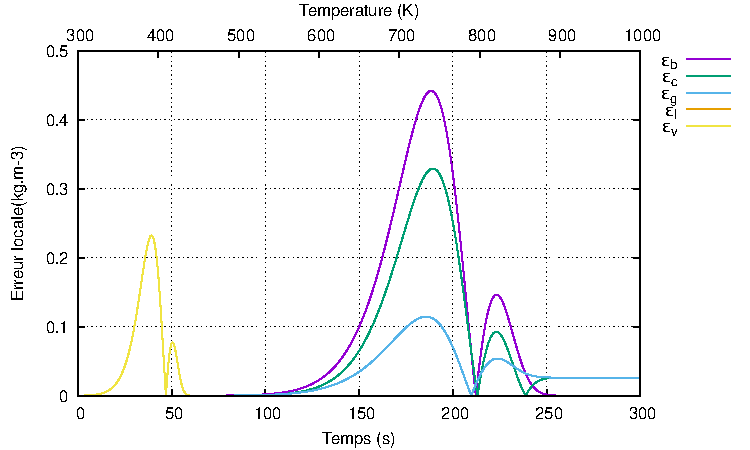
\includegraphics[width=0.75\linewidth]{images/error_EI.pdf}
    \caption{\centering \footnotesize Évolution des erreurs numériques locales sur les masses volumiques en fonction du temps (et de la température) pour le schéma de Euleur implicite }
    \label{fig:erEI}
\end{figure}


\begin{figure}[H]
    \centering
    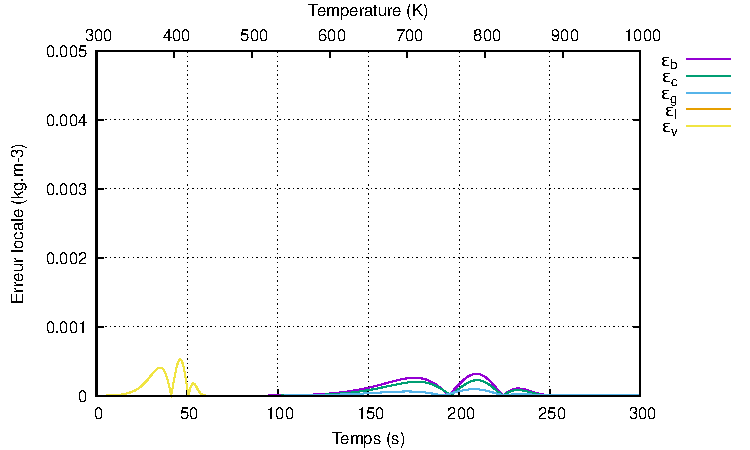
\includegraphics[width=0.75\linewidth]{images/error_CK2.pdf}
    \caption{\centering \footnotesize Évolution des erreurs numériques locales sur les masses volumiques en fonction du temps (et de la température) pour le schéma de Crank Nicolson. L'échelle de l'ordonnée est 100 fois plus petite que sur le graphe de l'erreur avec le schéma d'Euler)}
    \label{fig:erCK2}
\end{figure}

L'erreur devient plus importante aux moments où les masses volumiques varient le plus. Les ordres de grandeurs des erreurs numériques commises par les deux schémas sont incomparables: 0.1 kg.m$^{-3}$ pour Euler implicite, 0.0001 kg.m$^{-3}$ pour Crank-Nicolson. Cela est cohérent avec le fait que le schéma de Crank-Nicolson possède un ordre plus élevé (2) que Euler implicite (1). Les temps de calculs étant inférieurs à une seconde, le schéma de Crank-Nicolson est donc préférable.

\section{Partie chaleur}
Dans un premier temps on se limite à un cas unidimensionnel.
On utilise l'équation de la chaleur : 
\begin{equation}\label{eq:6}
\frac{\partial T}{\partial t} =    \frac{\lambda}{ \rho C_p} \frac{\partial^2 T}{\partial x^2} + Q_r
\end{equation}

On considère $ Q_r = 0$ , $\rho C_p = 1 $, $\lambda = 1$.  \\

On impose maintenant des conditions de Dirichlet aux limites : $\forall t$ on prend $ T(t, x=0) = T_0$ et $T(t, x=L) = T_0$. \\

\begin{tikzpicture}
    \draw (1,0) rectangle (4,1); % Dessine un rectangle de 5x3 cm
    \draw[<->] (1, 0.5) -- (4, 0.5);
    \node at (5, 0) {$T_0$};
    \node at (0, 0) {$T_0$};
    \node at (2.5, 0.8) {$L$};   
\end{tikzpicture}

Puis on choisit comme condition initiale, une condition de Cauchy : $T(t=0, x) = T_0 + T_{init}*sin(\pi\frac{x}{L})$.
On nous donne la solution analytique avec ces conditions :

$$ T(t,x)T_0+T_1*sin(\pi \frac{x}{L}esp(-D(\frac{\pi}{L})^2t) $$

Pour la suite, on prend $T_0=280K$, $T_{init}=800K$, et $L=1m$


Afin de résoudre l'équation, on utilise une méthode numérique avec 3 points en espace : 
\begin{equation}\label{eq:7}
    \frac{\partial^2 T_i}{\partial x^2} \simeq \frac{T_{i+1}+T_{i-1}-2T_i}{\Delta x^2}
\end{equation}
Puis, celle d'Euler implicite pour le temps :

$$ \frac{T_i^{n+1}-T_i^n}{\Delta t}= \frac{T_{i+1}^n+T_{i-1}^n-2T_i^{n+1}}{\Delta x^2} $$

\begin{equation}\label{eq:8}
    T_i^{n+1}=T_i^n + \frac{D\Delta t}{\Delta x^2} ( T_{i+1}^n-2T_i^n+T_{i-1}^n)
\end{equation}
Avec $D = \rho C_p$, $i$ représentent les indices d'espaces et $n$ les indices temporels.

On peut donc utiliser l'équation \eqref{eq:8} de façon numérique et ainsi approcher la solution réelle.

On note pour l'algorithme $nx $ le nombre d'intervalle en espaces, $t_{max}$ le temps maximal de la simulation.


\begin{tcolorbox}[colback=gray!10, colframe=black, boxrule=0.5pt]
\footnotesize
\begin{verbatim}

1. Initialisation

    Pour i de 1 à nx+1 :

        - Initialisation de chaque élément d'espace x_i avec leur température 
        - Initialisation de la température analytique

    Fin

    Affichage des valeurs pour verifier


2. Résolution

    Tant que t<t_max
    
        Pour i de 2 à nx
            - Mise en place des températures aux indices précédent et suivant 
            - Calcul de la nouvelle température affecté à une valeur temporaire
        Fin

        - Calcul des températures aux limites avec les conditions choisis 
        - Réaffectation des températures à partire de celles temporaires
        - ajout du pas de temps
        
    Fin


\end{verbatim}
\end{tcolorbox}


En prenant en compte la condition de Dirichlet, les valeurs précédentes et la solution analytique donnée on obtient ce graphique.

\begin{figure}[H]
    \centering
    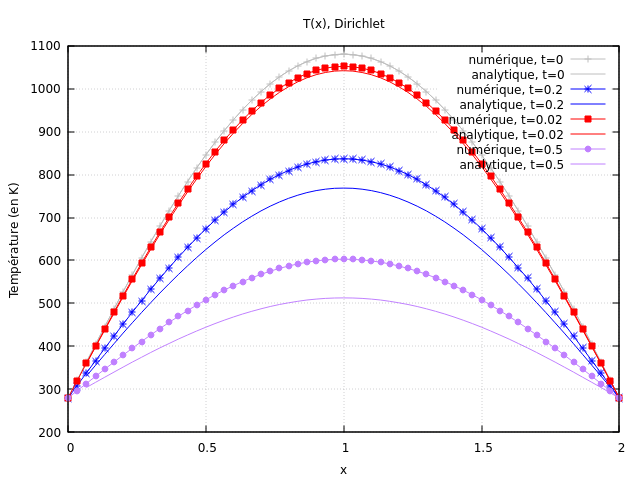
\includegraphics[width=0.8\linewidth]{images/graphe_temperature_grid.png}
    \caption{température le long d'un segment étudié en des temps différents avec la condition de Dirichlet}
\end{figure}

Il est possible de remarquer la décroissance au cours du temps. Ensuite, la différence entre la solution calculée numériquement et celle analytique s’accroît au fur et à mesure du fait que l'évolution de la température soit rapide. \\


Une fois les conditions de Dirichlet faites, on peut combiner celle de Dirichlet (à gauche) et celle de Neumann (à droite). 

On se place dans un milieu semi-infini vers la droite; cependant l'étude reste sur le domaine $[0;L]$. On impose pour tout $t$ $$T(t,x=0)=T_{init} $$ $$
\frac{\partial T}{\partial x}]_{x=L} = 0$$
On pose aussi la condition initiale  $$T(t=0, 0<x\leq L)=T_0 $$
La solution analytique donnée est $$ T(t,x) = (T_{init}-T_0)* erfc(\frac{x}{2\sqrt{Dt}})+T_0 $$

On reprend le même algorithme que précédemment. Une fois les conditions changées on peut tracer la courbe de température pour différents temps :

\begin{figure}[H]
    \centering
    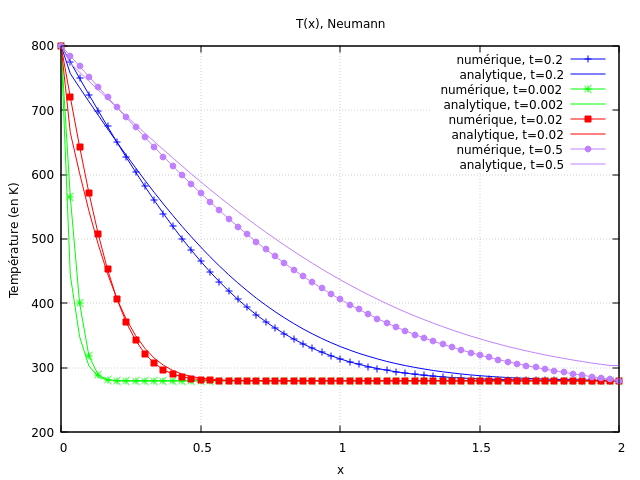
\includegraphics[width=0.8\linewidth]{images/graphe_temperature_Neumann_titre_grid.png}
    \caption{Température pour différent temps avec la condition de Neumann}
    \label{fig:enter-label}
\end{figure}

On voit l'augmentation de la température au cours du temps. De plus, la solution analytique admet des valeurs croissantes; elles sont visible car le domaine est semi-infini. On remarque aussi l'augmentation de l'écart entre la solution analytique et numérique qui augmente pour des $x>0.5$. Dans le domaine $[0;0.5]$ on remarque que la solution numérique est d'abord supérieure à celle analytique puis elle est supérieure.\\

En outre, il est sûrement préférable d'utiliser des conditions de Dirichlet-Neumann pour modéliser l'équation \eqref{eq:6} et surtout pour la pyrolyse. La condition de Dirichlet représente la température qui active le phénomène tandis que celle de Neumann traduit l'absence de perte de chaleur.

\section{Couplage}

Afin d'établir un schéma numérique pour le couplage, il est nécessaire de reprendre l'équation de la chaleur sous forme complète.


\begin{equation}\label{eq:chaleur}
\rho C_p\frac{\partial T}{\partial t} =    \nabla(\lambda\nabla T) + Q_r
\end{equation}

où T (K), $\lambda$ $(W/(m.K))$, $\rho$ $(kg/m^3)$ et $C_p$ $(J/(kg.K))$ désignent respectivement la température, la conductivité, la masse volumique et la chaleur spécifique.

Dans le cadre d'un couplage entre la chimie et la diffusion de la chaleur, les coefficients $\rho, C_p$ et $\lambda$ ne sont plus considérés comme constants au cours du temps. L'EDP devient alors non linéaire, car ces termes sont eux-mêmes fonction de la solution T. \\

\subsection{Cas unidimensionnel} Pour une résolution unidimensionnelle, il est possible de construire un schéma en utilisant un maillage régulier en espace de $Nx + 2$ points, c'est-à-dire $\forall x_i,\; i \in \{0, \dots, Nx+1\}$. La discrétisation en espace repose sur le principe suivant :
\begin{itemize}
    \item Approximation du flux thermique \( \lambda \frac{\partial T}{\partial x} \) aux milieux des mailles (entre $x_{i+1/2}$ et $x_{i-1/2}$).
    \item Calcul de la dérivée de ce flux en faisant la différence entre les flux à gauche et à droite d’un point.
    \item Utilisation de la moyenne harmonique pour traiter les termes fictifs de la conductivité en $i\pm1/2$.
  \end{itemize}

\vspace{0.5cm}
Pour le traitement temporel, des méthodes implicites sont privilégiées afin de garantir la stabilité du schéma, spécifiquement dans ce contexte non linéaire. De plus, les méthodes implicites permettent d'étudier l'évolution de la solution sur des temps longs (car pas de condition CFL), ce qui est crucial pour évoluer le sens physique d'une réaction comme la pyrolyse. Cependant, les termes non linéaires sont traités de manière explicite, dû à leur dépendance à la solution T. Ce couplage implicite au niveau de la température mais explicite au niveau de la chimie permet de garantir la stabilité tout en conservant un schéma numérique simple.\\


Pour le cas unidimensionnel, le couplage sera effectué avec différentes conditions initiales et aux limites :

\begin{itemize}
    \item \textbf{Condition initiale} : 
    \[
    T(0,x) = T_{\text{init}}(x) = 300 K
    \]

    \item \textbf{Condition de Dirichlet à gauche} : 
    \[
    T(t, x=0) = T_G = 800 K
    \]
    \[
    T_0^n = T_g(t),\quad  \forall n
    \]


    \item \textbf{Condition de Neumann adiabatique à droite} (pas de flux thermique) :
    \[
    \left. \frac{\partial T}{\partial x} \right|_{x = L} = 0 
    \]
    \[
    T_{Nx+1}^n = T_{Nx}^n \quad \forall n  
    \]
\end{itemize}

En suivant le procédé décrit précédemment, on obtient le schéma numérique d'Euler implicite à 3 points
\subsubsection*{Schéma d'Euler implicite à 3 points}
\begin{equation}
    \large
    - \beta_{i-1}^{n} T_{i-1}^{n+1} + (1 + \alpha_i^n) T_i^{n+1} - \beta_{i+1}^{n} T_{i+1}^{n+1} = T_i^n + \gamma_i^n Q_i^n, \quad i \in [|1, imax|]
\end{equation}

avec :
\[
\beta_{i \pm 1}^{n} = \frac{\Delta t}{\Delta x^2} \frac{\lambda_{i \pm \frac{1}{2}}^n}{(\rho C_p)_i^n}, \quad \quad\lambda_{i \pm \frac{1}{2}}^n = \frac{2\lambda_i \lambda_{i\pm1}}{\lambda_{i}+\lambda_{i\pm1}}
\]

\[
\alpha_i^n = \frac{\Delta t}{\Delta x^2 (\rho C_p)_i^n} \left( \lambda_{i - \frac{1}{2}}^n + \lambda_{i + \frac{1}{2}}^n \right)
\]

\[
\gamma_i^n = \frac{\Delta t}{(\rho C_p)_i^n}
\]

Il est possible de discrétiser ce système sous forme matricielle avec la méthode MOL, ce qui revient alors à résoudre un système d'équations différentielles ordinaires de la forme :

\begin{equation}
    (I + A) \cdot T^{n+1} = b
\end{equation}

où A est une matrice tridiagonale et b le second membre:

\[
A =
\begin{bmatrix}
\alpha_1^n & -\beta_2^n & 0 & \cdots & 0 \\
-\beta_1^n & \alpha_2^n & -\beta_3^n & \cdots & 0 \\
0 & \ddots & \ddots & \ddots & 0 \\
\vdots & \cdots & -\beta_{Nx-2}^n & \alpha_{Nx-1}^n & -\beta_{Nx}^n \\
0 & \cdots & 0 & -\beta_{Nx-1}^n & \beta_{Nx}^n
\end{bmatrix}
,\quad
b =
\begin{bmatrix}
    T_1^n + \beta_{0}^n T_G + \gamma_1^nQ_1^n \\
    T_2^n + \gamma_2^nQ_2^n  \\
    \vdots \\
    \vdots \\
    T_{Nx}^n + \gamma_{Nx}^nQ_{Nx}^n 
    
\end{bmatrix}
\]

Le dernier terme de la matrice et le premier terme du second membre prennent en compte les conditions aux limites de Dirichlet et Neumann, en effet :

\begin{align*}
    &\textbf{Pour i = 1 (Dirichlet : $T_0^{n+1}=T_G$)}: \\
    &- \beta_0^n T_0^{n+1} + (1 + \alpha_1^n) T_1^{n+1} - \beta_2^n T_2^{n+1} = T_1^n + \gamma_1^n Q_1^n  \\
    & \Longleftrightarrow   (1 + \alpha_1^n) T_1^{n+1} - \beta_2^n T_2^{n+1} = T_1^n + \beta_0^n T_g + \gamma_1^n Q_1^n  \\
    &\\
    &\textbf{Pour i = Nx (Neumann: $ T_{Nx+1}^{n+1} = T_{Nx}^{n+1}$}): \\
    & - \beta_{Nx-1}^n T_{Nx-1}^{n+1} + \left(1 + \alpha_{Nx}^n\right) T_{Nx}^{n+1} -  \beta_{Nx+1}^n T_{Nx+1}^{n+1} = T_{Nx}^n + \gamma_{Nx}^n Q_{Nx}^n \\
    & \Longleftrightarrow - \beta_{Nx-1}^n T_{Nx-1}^{n+1} + \left(1 +\beta_{Nx}^n \right) T_{Nx}^{n+1} = T_{Nx}^n + \gamma_{Nx}^n Q_{Nx}^n
\end{align*}

Le schéma en espace est d'ordre 2, tandis que le schéma en temps est d'ordre 1.


\subsubsection*{Schéma de Crank Nicolson à 3 points}

De la même manière qu'avec Euler implicite, le schéma de Crank-Nicolson à 3 points (Ordre 2 global) s'écrit comme suit :
\[
- \frac{\beta_{i-1}^{n}}{2} T_{i-1}^{n+1} + \left(1 + \frac{\alpha_i^n}{2} \right) T_i^{n+1} - \frac{\beta_{i+1}^n}{2} T_{i+1}^{n+1} =
\frac{\beta_{i-1}^n}{2} T_{i-1}^{n} + \left(1 - \frac{\alpha_i^n}{2} \right) T_i^{n} + \frac{\beta_{i+1}^n}{2} T_{i+1}^{n} + \gamma_i^n Q_i^n
\]

Sous forme matricielle, le système linéaire d'EDO suivant est obtenu.

\[
(I + \frac{1}{2}A) \cdot T^{n+1} = (I - \frac{1}{2}A) \cdot T^n + \gamma^n \cdot Q^n 
\]


D'un point de vue numérique, une procédure Fortran \texttt{save\_temp} est utilisée pour générer les solutions numériques jusqu'à un temps $t_{max}$ (avec une certaine fréquence nommée $freq$). L'algorithme général en pseudo code se présente de la manière suivante.

\begin{tcolorbox}[colback=gray!10, colframe=black, boxrule=0.5pt]
\footnotesize
\begin{verbatim}

save_temp(schema, ci, cl, L, nx, tmax, type_bois, cfl, freq)

1. Initialisation :
    - Calcul des propriétés du bois (humidité, masses volumiques)
    - Initialisation des vecteurs de masse volumiques
    - dx = L / (nx + 1)
    - dt selon le schéma (CFL si explicite, fixe sinon)
    - T(i) = Tinit(xi) pour i = 1 à nx
      T(0) = condition à gauche (Dirichlet)
    - Calcul des constantes de réaction k (Arrhenius)

2. Schéma numérique
Tant que tn < tmax :

    Pour i de 0 à nx+1 :
        - Calcul de rhoCp(i), lambda(i), Qr(i)
    fin
    
    Selon le schéma choisi :
        Schéma 1 (Euler explicite) :
            Pour i de 0 à nx+1 :
               - Résolution explicite
            fin
        Schéma 2 (Euler implicite) :
            - Remplissage matrice A
            - Construction second membre b avec T et Qr
            - Condition de Dirichlet dans b
            - Résolution A * Tnew = b
            - Application des CL (Neumann adiabatique)

        Schéma 3 (Crank-Nicolson) :
            - Calcul des matrices A1 et A2
            - Même principe qu’avec EI
            
    
    Pour i de 0 à nx+1 :
        - Calcul de knew avec Tnew
        - Mise à jour des masses volumiques avec CK2_step
        - Enregistrement des données au temps tn 
    fin

    - T = Tnew
    - tn = tn + dt 
    - k = knew

fin

Affichage du temps de calcul grâce à cpu_time()
\end{verbatim}
\end{tcolorbox}

Cet algorithme pour la résolution numérique de l'équation \eqref{eq:chaleur} utilise donc une méthode dite de splitting, où l'actualisation des températures se fait avant l'actualisation des masses volumiques pour un temps fixé. Cela est permis par le caractère semi-implicite du schéma, où les paramètres de la chimie au temps $t_n$ sont utilisés pour calculer les températures en $t_{n+1}$ avec le schéma numérique, cette dernière permettant ultérieurement de calculer les masses volumiques en $t_{n+1}$. La résolution des systèmes linéaires est faite avec un solveur LU adapté aux matrices creuses tridiagonales.\\

Le programme exporte pour un temps $t_n$ les températures et masses volumiques en chaque point $x_i$ du maillage. Les solutions sont générées pour les paramètres :
\begin{itemize}
    \item L = 0.2 m
    \item Nx = 128
    \item $\Delta t$ = 0.01 s
    \item $t_{max}$ = 200 s
    \item type\_bois = 1 (Chêne)
\end{itemize}

Pour le schéma de Crank-Nicolson, l'animation suivante peut être tracée :

\begin{figure}[H]
    \animategraphics[autoplay, loop, width=\linewidth, controls]{5}{images/1D/temp_}{01}{41}
    \caption{\centering Évolution de la température et des masses volumiques en 1D avec Crank-Nicolson}
\end{figure}

Le graphique montre bien une corrélation cohérente entre la température et les masses volumiques. En effet, une diminution importante de $\rho_b$ est observée à gauche du domaine, cela est dû à la condition de Dirichlet qui maintient cette extrémité à 800 K. Le phénomène de pyrolyse, qui se produit au-delà des 600 K, est alors mis en exergue par la formation de charbon et de gaz à gauche du domaine (augmentation des masses volumiques). Cependant, le front de chaleur semble se déplacer bien plus rapidement que le front de pyrolyse. De plus, la propagation du front de chaleur marque la vaporisation du liquide présent dans le bois (vers 373 K), avec une diminution de liquide au détriment de la vapeur. \\

Le graphique confirme le sens physique de la résolution, bien qu'on puisse facilement observer l'effet de la température sur la partie chimie, il est difficile de visualiser l'inverse. Pour mieux comprendre l'intrication entre ces deux aspects du schéma, la résolution dans un cas bidimensionnel est préférable.

\subsection{Cas bidimensionnel}

La construction d'un schéma pour l'équation de la chaleur en 2D ne change pas significativement par rapport au cas unidimensionnel, le stencil comporte une dimension de plus caractérisée par l'index j, avec 2 points qui viennent s'ajouter. Le schéma d'Euler implicite s'écrit alors :

\begin{equation}\label{CouplageEI2D}
    (1 + \alpha_{i,j}^n) T_{i,j}^{n+1} = T_{i,j}^{n} + \beta_{i+1}^{n} T_{i+1,j}^{n+1} + \beta_{i-1}^{n} T_{i-1,j}^{n+1} + \beta_{j+1}^{n} T_{i,j+1}^{n+1} + \beta_{j-1}^{n} T_{i,j-1}^{n+1} + \gamma_{i,j}^n Q_{i,j}^n
\end{equation}

\[
\beta_{i\pm1}^n = \frac{\Delta t}{\Delta x^2} \frac{\lambda_{i \pm \frac{1}{2}, j}^n}{(\rho C_p)_{i,j}^n}
\qquad
\beta_{j\pm1}^n = \frac{\Delta t}{\Delta y^2} \frac{\lambda_{i, j \pm \frac{1}{2}}^n}{(\rho C_p)_{i,j}^n}
\]

\[
\alpha_{i,j}^n = \beta_{i-1}^n + \beta_{i+1}^n + \beta_{j-1}^n + \beta_{j+1}^n
\qquad
\gamma_{i,j}^n = \frac{\Delta t}{(\rho C_p)_{i,j}^n}
\]

Pour la résolution d'un tel système, une méthode itérative sera privilégiée. En effet, le remplissage d'une matrice pour le cas 2D devient très complexe, car c'est une matrice pentadiagonale ou par blocs, qui demande un nouveau solveur. De plus, la résolution de ce système revient à changer toute l'architecture du code. De ce fait, la méthode de Gauss-Seidel est employée, elle consiste à mettre à jour les valeurs inconnues une par une, en utilisant les dernières valeurs disponibles dès qu’elles sont calculées. \\

Concrètement, l'ensemble du maillage en espace est parcouru (ligne par ligne), et la température $T_{i,j}$ est mise à jour en fonction des valeurs de ses voisins. Ces valeurs sont alors directement utilisées pour calculer les valeurs voisines. \\

Ce processus est répété plusieurs fois jusqu’à ce que la solution ne change presque plus d’une itération à l’autre, c’est-à-dire que l’erreur entre deux itérations devienne très petite (ici, on s’arrête si l’erreur est inférieure à $10^{-6}$). Cette méthode se base donc sur des hypothèses de convergence sur la solution (ce qui n'est pas toujours le cas), mais elle reste particulièrement utile dans la résolution d'une EDP non linéaire en 2D comme celle-ci. La procédure permettant de générer les solutions \texttt{save\_temp\_2D} se calque sur le cas unidimensionnel, en ajoutant les paramètres de la deuxième dimension (j, $\Delta y$ Ly, Ny) et en augmentant le rang des différents tenseurs (T, Tnew, k, $\lambda$, $\rho$...) . \\

Similairement par rapport à la 1D, les données sur la température et les masses volumiques en tous points (i,j) sont calculées, en utilisant les conditions initiales et aux limites suivantes :


\begin{center}
\begin{tikzpicture}[scale=0.65]

\def\nx{12}
\def\ny{9}
\def\dirStart{3}
\def\dirEnd{6.75}

\draw[step=0.8cm,gray!30,very thin] (0,0) grid ({(\nx+1)*0.8},{(\ny+1)*0.8});

\draw[very thick] (0,0) rectangle ({(\nx+1)*0.8},{(\ny+1)*0.8});

\draw[line width=3pt,red] (0,{0.7*\dirStart}) -- (0,{0.9*\dirEnd});
\node[red,rotate=90,anchor=south] at (-0.4,{0.8*(\dirStart+\dirEnd)/2}) {$\boxed{T = 1000\,\text{K}}$};

\draw[line width=2pt,blue] (0,0) -- (0,{0.7*\dirStart});
\draw[line width=2pt,blue] (0,{0.9*\dirEnd}) -- (0,{0.8*(\ny+1)});
\draw[line width=2pt,blue] ({0.8*(\nx+1)},0) -- ({0.8*(\nx+1)},{0.8*(\ny+1)});
\draw[line width=2pt,blue] (0,0) -- ({0.8*(\nx+1)},0);
\draw[line width=2pt,blue] (0,{0.8*(\ny+1)}) -- ({0.8*(\nx+1)},{0.8*(\ny+1)});

\node[blue,rotate=90] at ({0.8*(\nx+1)+0.5},{0.8*(\ny+1)/2}) {\large $\frac{\partial T}{\partial x} = 0$};
\node[blue] at ({0.8*(\nx+1)/2},-0.5) {\large $\frac{\partial T}{\partial y} = 0$};
\node[blue] at ({0.8*(\nx+1)/2},{0.8*(\ny+1)+0.5}) {\large $\frac{\partial T}{\partial y} = 0$};

\node at ({0.8*(\nx+1)/2},{0.8*(\ny+1)/2}) {\textbf{Condition initiale} : $T_0 = 300\,\text{K}$};

\draw[->,thick] (-0.2,0) -- ({0.8*(\nx+1)+0.5},0) node[right] {$x$};
\draw[->,thick] (0,-0.2) -- (0,{0.8*(\ny+1)+0.5}) node[above] {$y$};

\node at ({0.8*(\nx+1)},-0.5) {$nx+1$};
\node at (-1,{0.8*(\ny+1)}) {$ny+1$};

\end{tikzpicture}
\end{center}

La condition de Dirichlet permet de bien visualiser la diffusion en 2D, car la diffusion se fera de manière diffuse et isotrope. Le visualisation des données se fait sous forme de heatmap, qui est particulièrement utile pour les cas 2D et spécifiquement pour la diffusion de la chaleur. Sur une même animation, l'évolution des champs de température et de la masse volumique du charbon dans le domaine est représentée.
\begin{figure}[H]
    \makebox[\textwidth][c]{
        \animategraphics[autoplay,loop,controls,width=1.2\textwidth]{5}{images/2D/multiplot_}{01}{41}
    }
    \caption{\centering Évolution des champs de température et de masse volumique du charbon en 2D jusqu'à $t_{max} = 200$ s.}
\end{figure}

L'évolution de la température dans le bois est cohérente. La condition de Dirichlet imposée à 1000 K sur une portion du domaine gauche induit bien une propagation de chaleur de manière diffuse et isotrope. Pour la condition de Neumann adiabatique, elle garantit "l'isolation" du domaine en nullifiant le flux de chaleur au bord. Le graphique à droite montrant l'évolution de $\rho_c$ est cohérente avec le profil de la température à gauche, avec une formation de charbon isotrope à gauche quand la température dépasse les 600 K. Similairement au cas 1D, le front de chaleur se propage plus rapidement et de manière plus diffuse que le front de pyrolyse. Celui-ci reste très restreint à gauche avec un net clivage par rapport au reste du domaine. \\

Maintenant que le schéma est validé pour le cas bidimensionnel, un problème différent, qui permet de visualiser l'impact de la chimie sur la chaleur, peut être étudié. Pour ce faire, un domaine comportant deux essences de bois différentes est étudié, avec en bas un bois dense comme le chêne et en haut un bois moins dense, à l'instar du pin. La propagation de la chaleur devient alors anisotrope et non uniforme, en raison des différences de diffusivité thermique entre les deux essences \cite{1}. Le pin, moins dense, présente une diffusivité thermique $D = \frac{\lambda}{\rho C_p}$ plus élevée que le chêne. Le front thermique progresse donc plus vite en haut qu’en bas, créant une dissymétrie dans la diffusion. Il en résulte une zone angulaire, dans le coin inférieur, qui reste plus froide plus longtemps. Ce problème avec les différentes conditions peut se visualiser de la manière suivante :

\begin{center}
\begin{tikzpicture}[scale=0.7]

\def\nx{12}
\def\ny{9}
\def\dirStart{0}
\def\dirEnd{\ny+1}

\draw[step=0.8cm,gray!30,very thin] (0,0) grid ({(\nx+1)*0.8},{(\ny+1)*0.8});

\draw[very thick] (0,0) rectangle ({(\nx+1)*0.8},{(\ny+1)*0.8});

\draw[line width=3pt,red] (0,{0.8*\dirStart}) -- (0,{0.8*\dirEnd});
\node[red,rotate=90,anchor=south] at (-0.4,{0.8*(\dirStart+\dirEnd)/2}) {\large $\boxed{T = 1000\,\text{K}}$};

\draw[line width=2pt,blue] ({0.8*(\nx+1)},0) -- ({0.8*(\nx+1)},{0.8*(\ny+1)});
\draw[line width=2pt,blue] (0,0) -- ({0.8*(\nx+1)},0);
\draw[line width=2pt,blue] (0,{0.8*(\ny+1)}) -- ({0.8*(\nx+1)},{0.8*(\ny+1)});

\node[blue,rotate=90] at ({0.8*(\nx+1)+0.5},{0.8*(\ny+1)/2}) {\large $\frac{\partial T}{\partial x} = 0$};
\node[blue] at ({0.8*(\nx+1)/2},-0.5) {\large $\frac{\partial T}{\partial y} = 0$};
\node[blue] at ({0.8*(\nx+1)/2},{0.8*(\ny+1)+0.5}) {\large $\frac{\partial T}{\partial y} = 0$};

\draw[dashed,thick] (0,{0.8*(\ny+1)/2}) -- ({0.8*(\nx+1)},{0.8*(\ny+1)/2});

\node at ({0.8*(\nx+1)/2},{0.8*(\ny+1)*3/4}) {\textbf{Bois de pin, $T_0 = 300\,\text{K}$}};
\node at ({0.8*(\nx+1)/2},{0.7*(\ny+1)*3/4}) {\textbf{$\rho_{b,0} = 360\,\text{kg/m$^3$} $}};
\node at ({0.8*(\nx+1)/2},{0.8*(\ny+1)*1/4}) {\textbf{Bois de chêne, $T_0 = 300\,\text{K}$}};
\node at ({0.8*(\nx+1)/2},{0.5*(\ny+1)*1/4}) {\textbf{$\rho_{b,0} = 888\,\text{kg/m$^3$} $}};
\draw[->,thick] (-0.2,0) -- ({0.8*(\nx+1)+0.5},0) node[right] {$x$};
\draw[->,thick] (0,-0.2) -- (0,{0.8*(\ny+1)+0.5}) node[above] {$y$};
s
\node at ({0.8*(\nx+1)},-0.5) {$nx+1$};
\node at (-1,{0.8*(\ny+1)}) {$ny+1$};

\end{tikzpicture}
\end{center}

Les solutions suivantes sur le champ de température sont alors obtenues en utilisant un programme similaire :

\begin{figure}[H]
    \animategraphics[autoplay, loop, width=\linewidth, controls]{5}{images/2D_2W/temp_}{01}{41}
\end{figure}

Comme prévu, le caractère anisotrope de la diffusion est souligné par l'animation, avec une diffusion de la chaleur qui se fait plus rapidement en haut (dans le pin) qu'en bas (dans le chêne). Cela corrobore les résultats obtenus dans l'étude de D.K Shen et al. \cite{1}, où la température de surface du chêne augmentait moins au cours du temps par rapport à des bois moins denses comme le mélèze ou le tremble. \\

Néanmoins, ce contraste n'est pas réellement marquant car on s'intéresse à deux espèces d'un même matériau qui est le bois, i.e. leur diffusivité est relativement proche considérant l'ensemble des matériaux existants. Une étude sur des matériaux aux propriétés différentes mettrait davantage cet effet en avant, mais cela sortirait du cadre physique de notre modèle (notamment au niveau des équations de transfert de masse).
\section{Conclusion}


Ce projet a permis de modéliser et de simuler numériquement le phénomène de pyrolyse du bois, dans un premier temps en s'intéressant séparément au transfert de masse et à la diffusion de la chaleur, avant de coupler ces aspects pour avoir un modèle plus global du processus physique. L'utilisation de schémas implicites, tels que Euler implicite et Crank-Nicolson, a permis d'étudier l'évolution des champs de température et des masses volumiques dans des cas unidimensionnels et bidimensionnels. \\

Les résultats illustrent le phénomène de pyrolyse, par la formation de gaz et de charbon dans les zones de forte température. Le cas bidimensionnel a été rendu possible grâce à l'utilisation de la méthode de résolution de système itératif de Gauss-Seidel. Enfin, l'étude en deux dimensions avec des conditions aux limites bien choisies a mis en exergue l'intrication qui règne entre la diffusion de la chaleur et le transfert de masse.

\newpage
\section{Annexes}
Ci-dessous des bouts de code en Fortran qui contiennent des procédures importantes pour ce TER, notamment celles calculant les nouvelles masses volumiques au temps n+1 ainsi que la procédure du programme principal permettant de construire nos données. Pour des raisons de clarté, la création des données pour Crank-Nicolson est omise car elle ressemble fortement à celle d'Euler.

\vspace{0.5cm}
\begin{lstlisting}[caption={Procédure \texttt{Euler\_step}}, label={lst:euler_step}]
subroutine Euler_step(rho, k, dt)

    real(PR), dimension(:), intent(inout)   :: rho, k
    real(PR), intent(in)                    :: dt

    rho(1) = rho(1)/(1._PR + dt * (k(1) + k(2)))
    rho(2) = rho(2) + dt * k(1) * rho(1)
    rho(3) = rho(3) + dt * k(2) * rho(1)
    rho(4) = rho(4)/(1._PR + dt * k(3))
    rho(5) = rho(5) + dt * k(3) * rho(4)

end subroutine Euler_step
\end{lstlisting}

\begin{lstlisting}[caption={Procédure \texttt{CK2\_step}}, label={lst:ck2_step}]
subroutine CK2_step(rho, k, k_new, dt)

    real(PR), dimension(:), intent(inout)   :: rho, k, k_new
    real(PR), intent(in)                    :: dt
    real(PR)                                :: rhob, rhol

    rhob = rho(1)
    rhol = rho(4)

    rho(1) = rho(1) * ((1._PR - dt/2._PR * (k(1) + k(2)))/(1._PR + dt/2._PR *(k_new(1) + k_new(2))))
    rho(2) = rho(2) + dt/2._PR * (k_new(1) * rho(1) + k(1) * rhob)
    rho(3) = rho(3) + dt/2._PR * (k_new(2) * rho(1) + k(2) * rhob)
    rho(4) = rho(4) * ((1._PR - dt/2._PR * k(3))/(1._PR + dt/2._PR * k_new(3)))
    rho(5) = rho(5) + dt/2._PR * (k_new(3) * rho(4) + k(3) * rhol)

end subroutine CK2_step
\end{lstlisting}

\begin{lstlisting}[caption={Procédure \texttt{create\_data\_Euler}}]
subroutine create_data_Euler(rho, k, t, tf, dt, Temp, Tempf)

    real(PR), dimension(:), intent(inout)   :: rho, k                   !Vecteurs contenant les masses volumiques et taux de reactions du systeme
    real(PR), intent(inout)                 :: t, tf, dt, Temp, Tempf   !temps (initialement 0), temps final, pas de temps, temperature (initialement 300K), temperature finale 
                                                                        !
    real(PR)                                :: t1, t2, alpha
    integer                                 :: N, i

    open(unit=101, file = "data/densite_Euler.dat")
    
    N = INT(tf/dt) !Calcul du nombres d'operations pour le schema

    alpha = (Tempf-Temp)/tf !Alpha est le coefficient directeur de T(t)
                            !Pour aller de la temperature initiale a finale en un temps tf (t0=0)

    call cpu_time(t1)
    do i = 1, N

        write(101,*) rho, t, Temp
        Temp = Temp + dt*alpha      !Calcul de la temperature au temps t_n+1

        call arrhenius(k, Temp)     !Calcul des coefficients k au temps t_n+1
                                    !avec la loi d'Arrhenius
                                    
        call Euler_step(rho, k, dt) !Un pas de temps avec le schema implicite d'Euler
                                    !calcul de rho_n+1
        t = t + dt
    
    end do
    
    call cpu_time(t2)
    print *, "Temps d'execution Euler-SI :", t2 - t1
    close(101)

end subroutine create_data_Euler
\end{lstlisting}

\subsection*{Étude de l'ordre pour le couplage 1D}
Dans le cadre du couplage en 1D, l'utilisation d'une extrapolation de Richardson est mise en place pour évaluer l'ordre des schémas d'Euler implicite et Crank-Nicolson. Cela consiste à diminuer successivement le pas de temps par 2, puis à comparer les rapports d'erreurs globales avec ces pas de temps. Seulement deux rapports d'erreurs ont pu être calculés pour chaque schéma, après cela un effet de plateau sur l'erreur s'amorce et fausse les résultats.

\begin{figure}[H]
    \centering
    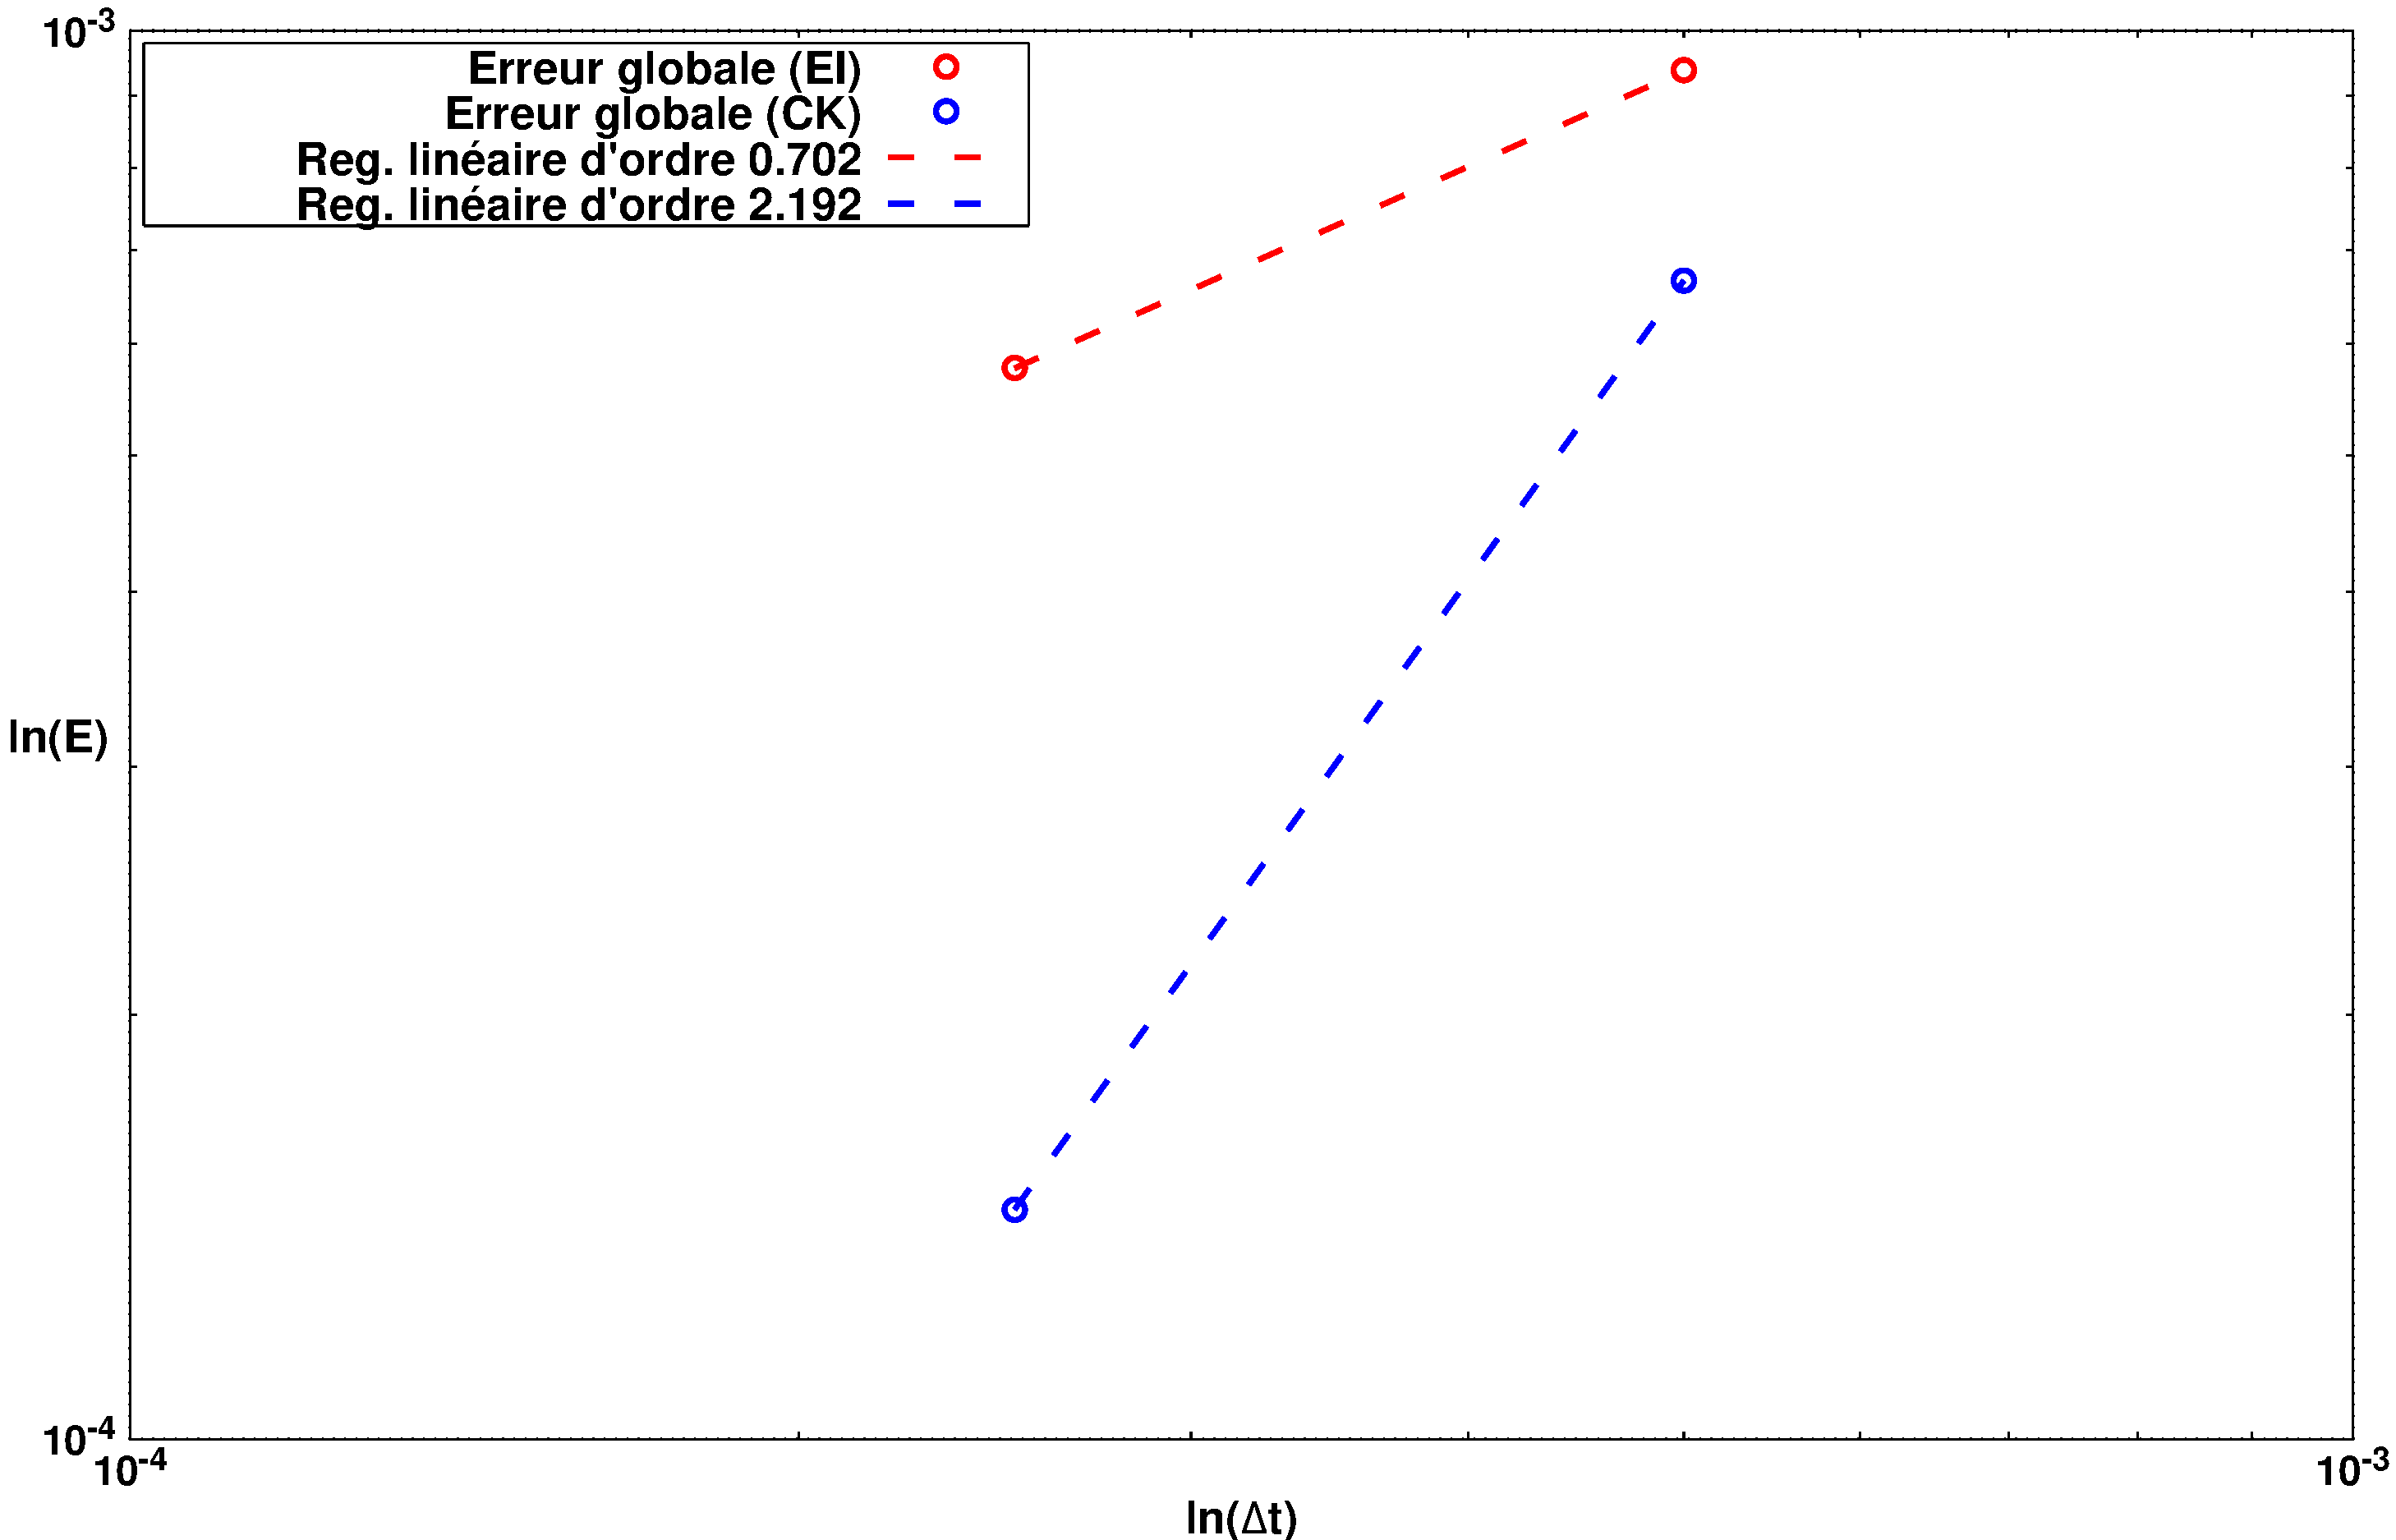
\includegraphics[width=0.8\linewidth]{images/ordre.pdf}
    \caption{Régression linéaire sur l'erreur globale en fonction du pas de temps en échelle logarithmique}
\end{figure}

Aux incertitudes des calculs près, les ordres théoriques des schémas sont approximés.
\newpage
\begin{thebibliography}{99}

    \addcontentsline{toc}{section}{Bibliographie}

    \bibitem{1} D.K. Shen et al, \textit{Modeling pyrolysis of wet wood under external heat flux}, Fire Safety Journal 42 (2007) 210–217

\end{thebibliography}

\end{document}